%%%%%%%%%%%%%%%%%%%%%%%%%%%%%%%%%%%%%%%%%
% fphw Assignment
% LaTeX Template
% Version 1.0 (27/04/2019)
%
% This template originates from:
% https://www.LaTeXTemplates.com
%
% Authors:
% Class by Felipe Portales-Oliva (f.portales.oliva@gmail.com) with template 
% content and modifications by Vel (vel@LaTeXTemplates.com)
%
% Template (this file) License:
% CC BY-NC-SA 3.0 (http://creativecommons.org/licenses/by-nc-sa/3.0/)
%
%%%%%%%%%%%%%%%%%%%%%%%%%%%%%%%%%%%%%%%%%

%----------------------------------------------------------------------------------------
%	PACKAGES AND OTHER DOCUMENT CONFIGURATIONS
%----------------------------------------------------------------------------------------

\documentclass[
	12pt, % Default font size, values between 10pt-12pt are allowed
	%letterpaper, % Uncomment for US letter paper size
	%spanish, % Uncomment for Spanish
]{fphw}

% Template-specific packages
\usepackage[utf8]{inputenc} % Required for inputting international characters
\usepackage[T1]{fontenc} % Output font encoding for international characters
\usepackage{mathpazo} % Use the Palatino font
\usepackage[dvipsnames]{xcolor}
\usepackage{graphicx} % Required for including images
\usepackage{amsmath}
\usepackage{booktabs} % Required for better horizontal rules in tables
\usepackage{listings} % Required for insertion of code
\usepackage{enumerate} % To modify the enumerate environment
\usepackage{ragged2e}
\usepackage{cancel}
\usepackage{MnSymbol,bbding,pifont}
\usepackage{everyhook}
\usepackage{lscape}
\usepackage{array}
\usepackage{float,graphicx}
\newcommand{\randomcolor}{%
  \definecolor{randomcolor}{RGB}
   {
    \pdfuniformdeviate 256,
    \pdfuniformdeviate 256,
    \pdfuniformdeviate 256
   }%
  \color{randomcolor}%
}

\usepackage{listings}
\usepackage[dvipsnames]{xcolor}
\definecolor{codegreen}{rgb}{0,0.6,0}
\definecolor{codegray}{rgb}{0.5,0.5,0.5}
\definecolor{codepurple}{rgb}{0.58,0,0.82}
\definecolor{backcolour}{rgb}{1,1,1}
\lstdefinestyle{mystyle}{
    backgroundcolor=\color{backcolour},   
    commentstyle=\color{codegreen},
    keywordstyle=\color{magenta},
    numberstyle=\tiny\color{codegray},
    stringstyle=\color{codepurple},
    basicstyle=\ttfamily\footnotesize,
    breakatwhitespace=false,         
    breaklines=true,                 
    captionpos=b,                    
    keepspaces=true,                 
    numbers=left,                    
    numbersep=5pt,                  
    showspaces=false,                
    showstringspaces=false,
    showtabs=false,                  
    tabsize=2
}
\renewcommand{\lstlistingname}{Código}% Listing -> Algorithm
\lstset{style=mystyle}

%----------------------------------------------------------------------------------------
%	ASSIGNMENT INFORMATION
%----------------------------------------------------------------------------------------

\title{Assignment \#3} % Assignment title

\author{Luis Alberto Ballado Aradias} % Student name

\date{\today} % Due date

\institute{Centro de Investigación y de Estudios Avanzados del IPN \\ Unidad Tamaulipas} % Institute or school name

\class{Introducción al Análisis de Fourier (Sep - Dec 2022)} % Course or class name

\professor{Dr. Wilfrido Gómez-Flores} % Professor or teacher in charge of the assignment

%----------------------------------------------------------------------------------------


\begin{document}

\maketitle % Output the assignment title, created automatically using the information in the custom commands above

%----------------------------------------------------------------------------------------
%	ASSIGNMENT CONTENT
%----------------------------------------------------------------------------------------

{\color{teal}
  \dotfill
  PULSO RECTANGULAR
\dotfill}

\[f(t) =\left\{ \begin{array}{lr}1, & \lvert t \rvert < \frac{\tau}{2} \\0, & \lvert t \rvert  > \frac{\tau}{2} \end{array}\right.\]

\begin{figure}[H]
  \centering
  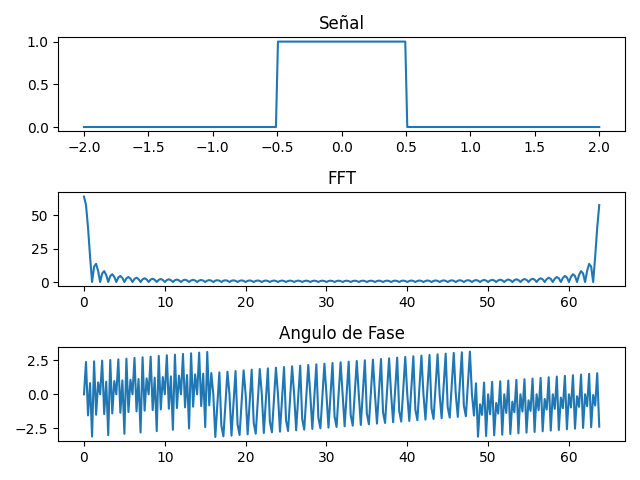
\includegraphics[scale=0.8]{images/pulso_rectangular.png}
\end{figure}


\newpage

{\color{teal}
  \dotfill
  ESCALON UNITARIO
\dotfill}

\[f(t) =\left\{ \begin{array}{lr}1, &  t > 0 \\0, & t < 0 \end{array}\right.\]

\begin{figure}[H]
  \centering
  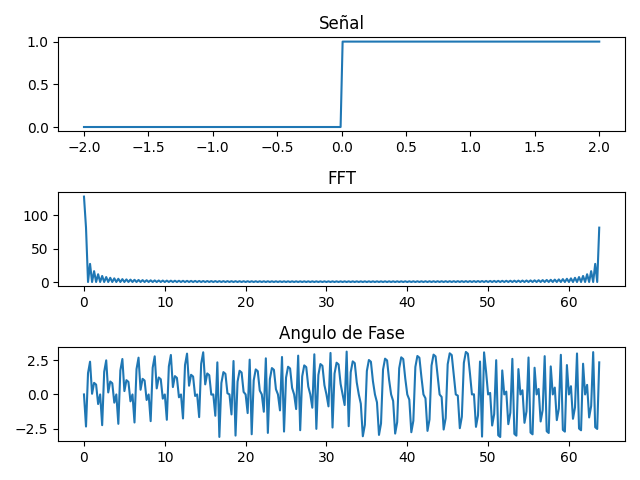
\includegraphics[scale=0.8]{images/escalon_unitario.png}
\end{figure}

\newpage

{\color{teal}
  \dotfill
  EXPONENCIAL
\dotfill}

\[f(t) =\left\{ \begin{array}{lr} e^{-at}, & t > 0 \\0, & t < 0 \end{array}\right.\]

\begin{figure}[H]
  \centering
  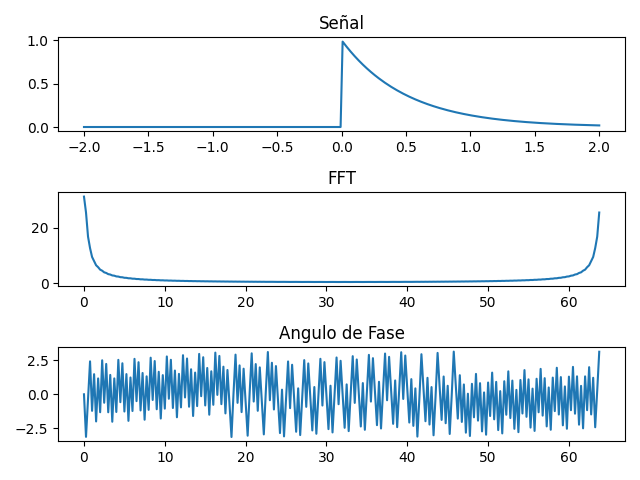
\includegraphics[scale=0.8]{images/exponencial.png}
\end{figure}

\newpage

{\color{teal}
  \dotfill
  FUNCION A
\dotfill}

\[f(t)=5+2*cos(2*\pi *t -\pi/2)+3*cos(4*\pi *t)\]

\begin{figure}[H]
  \centering
  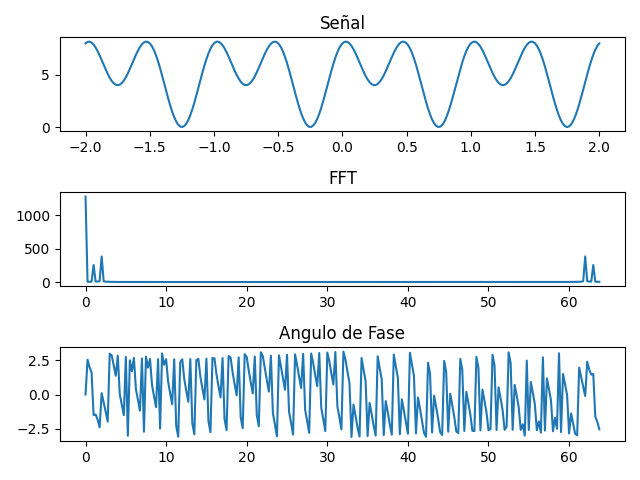
\includegraphics[scale=0.8]{images/funcion_a.png}
\end{figure}

\newpage

{\color{teal}
  \dotfill
  FUNCION B
\dotfill}

\[f(t)=5+8*cos(2*\pi *t - \frac{\pi}{2}) + 4*cos(4*\pi *t)+2*cos(8*\pi *t-\frac{\pi}{2})+cos(16*\pi *t)+\]
\[+2*cos(32*\pi *t - \frac{\pi}{2}) \]

\begin{figure}[H]
  \centering
  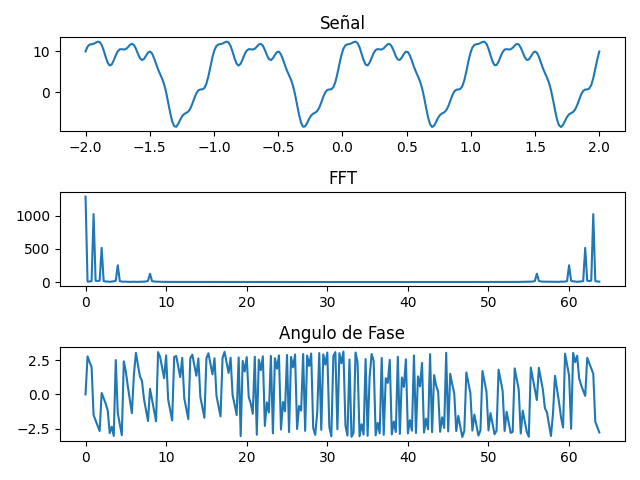
\includegraphics[scale=0.8]{images/funcion_b.png}
\end{figure}

\newpage
{\color{teal}
\dotfill
Código python
\dotfill}

\begin{lstlisting}[language=Python, caption=Dibujo de funciones]
def pulso_rectangular(t):
    '''PULSO RECTANGULAR'''
    return 1 * (abs(t) < 0.5)
    
def escalon_unitatio(t):
    '''ESCALON UNITARIO'''
    return 1 * (t >= 0)

def exponencial(t):
    '''FUNCION EXPONENCIAL'''
    alpha = randrange(3)
    return np.exp(-alpha * t) * (t > 0)

def funcion_a(t):
    '''FUNCION A'''
    return 5+2*np.cos((2*np.pi*t)-(np.pi/2)) + 3*np.cos(4*np.pi*t)

def funcion_b(t):
    '''FUNCION B'''
    return 5+8*np.cos((2*np.pi*t)-(np.pi/2))+4*np.cos(4*np.pi*t)+2*np.cos((8*np.pi*t)-(np.pi/2))+np.cos(16*np.pi*t)+2*np.cos((32*np.pi-(np.pi/2)))
\end{lstlisting}

\newpage
\begin{lstlisting}[language=Python, caption=FFT - radix2]
def FFT2(x):
    ''' radix-2 FFT '''
    x = np.array(x, dtype=float)
    N = int(x.size)
    n = np.log2(N)
    d = 1
    for i in range(1,int(n)):
        w = np.exp(-(1j*2*np.pi)/(2*d))
        for a in range(0,d-1):
            b = 0
            while(b<N-1):
                wa=pow(w,a)
                id1 = b+a+1
                id2 = b+d+a+1
                t_0 = x[id1] + (wa)*x[id2]
                t_1 = x[id1] - (wa)*x[id2]
                x[id1] = t_0
                x[id2] = t_1
                b = b+2*d
        
        d = 2*d
    return x
\end{lstlisting}

\begin{lstlisting}[language=Python, caption=Algoritmo Gold Rader]

def bit_reversal(data):
    '''
    gold rader - zero padding
    :param data: array de datos
    :return: array signal con zeros
    '''
    n = int(data.size)
    j = 0
    i = 0
    while i < n-1:
        k = n/2
        if (i<j):
            temp = data[int(i)]
            data[int(i)] = data[int(j)]
            data[int(j)] = temp
        while(k<=j):
            j = j-k
            k = k/2
        j = j+k
        i += 1        
    return data

\end{lstlisting}
%----------------------------------------------------------------------------------------

\end{document}
